\documentclass{jsarticle}
\usepackage[dvipdfmx]{graphicx}
\usepackage{listings,jlisting}
\usepackage{float}

\title{情報工学実験2 数理計画法 第三回}

\author{学生番号4617043 神保光洋}
\date{\today}
\begin{document}
\maketitle

\section{実験の要旨}
実験課題1で求めたビット誤り率$P_e$より誤り率を小さくする方法を
扱う。具体的には、実験課題2で作成したハミング符号を用いて実験課題1
と同様、繰り返しシュミレーションを行って誤り率(BER)$P_{dec}$を求める。

\section{実験の目的}
実験課題1で求めたビット誤り率$P_e$より誤り率を小さくする。

\section{実験の原理}
$(n, k) = (7, 4)$ ハミング符号を用いる。$(7, 4)$ ハミング符号とは
代表的な誤り訂正符号の一つであり、単一誤りの訂正を可能とする。
符号化と呼ばれる操作によって4ビットの情報を7ビットの符号語に
変換し、送信する。




\section{実験装置あるいは実験方法}
\subsection{実行環境}
Mojave 10.14.1
zsh 5.3 (x86\_64-apple-darwin18.0)
g++ 4.2.1

\subsection{実験手順}
\subsubsection{情報系列 $w = (w_1, w_2, ..., w_k)$の生成}
(課題1)
\subsubsection{符号語 $x = (x_1, x_2, ..., x_k)$の生成}
(課題2)
\subsubsection{BSCでの雑音$e = (e_1, e_2, ..., e_n)$の発生と受信系列$y=(y_1, y_2, ..., y_n)$の生成}
(課題1)
\subsubsection{ハミング符号の復号}
受信系列$y$から復号を行い、推定符号語$\hat {x} = (\hat{x_1},\hat{x_2}, ..., \hat{x_n})$,
推定情報系列$\hat {w} = (\hat{w_1},\hat{w_2}, ..., \hat{w_n})$を得る。
(課題2)

\subsubsection{誤りビット数の算出}
情報系列$w$と推定情報系列$\hat{w}$を比較し誤りビット率を求める
(n-kビットの冗長ビットは含めない)
(課題1)

\subsubsection{復号後のビット誤り率$P_dec$の計算}
$1~5$を十分な精度が得られるまで繰り返し(=SIM回、自分で適当な値に設定)、
復号後のビット誤り率$P_dec$を求める。
$P_dec$は誤った推定情報系列ビットの総数を送信した情報系列の
ビット総数(k * SIM)で割ったものある。
(課題1)
\subsubsection{1~6を$\epsilon$に対し実行する}

\section{結果}
結果は以下の様になった。

\begin{lstlisting}

➜ g++ Source.c && ./a.out
eps      P_e
0.001000 0.000015
0.002000 0.000040
0.003000 0.000085
0.004000 0.000198
0.005000 0.000278
0.006000 0.000260
0.007000 0.000395
0.008000 0.000500
0.009000 0.000682
0.010000 0.000847

\end{lstlisting}


誤り率の結果と理論値は以下のグラフの様になった。
\begin{figure}[H]
  \centering
  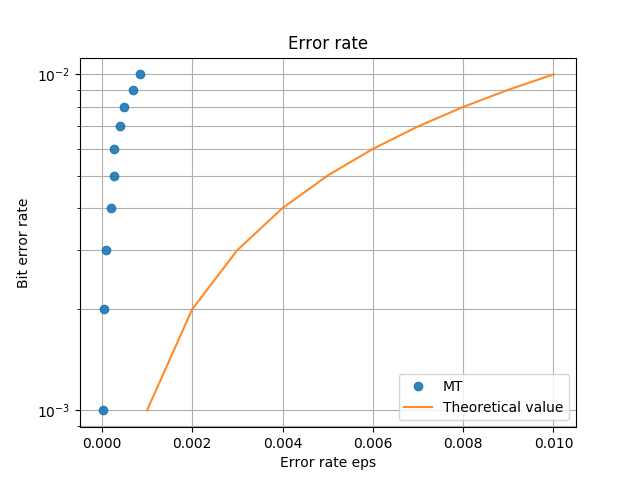
\includegraphics[width=12cm]{./graph1.png}
  \caption{誤り率の結果と理論値}
\end{figure}


\section{検討・考察}
\subsection{検討事項3-1}
$\epsilon$が小さいとき、シュミレーションが少ないとBERが
0となり正しく計測できない場合がある。
0より大きいBERを計測するにはどの程度のシュミレーション
回数を実行する必要があるか。

情報工学実験2情報シュミレーション第一回目の検討同様
少なくとも100000回は必要であると検討される。

\subsection{検討事項3-2}
ハミング符号を用いたとき、BERがどのように変化するか理論的に考察せよ。

グラフ1よりグラフ1は対数グラフをとっているが、
$P_{dec}$の値は直線的に変化していることが考察される。これは
理論値と比べるとより明らかである。
したがってBERの変化は誤り率を$e$とすると
$r \in R$を用いて
$$P_dec = r^e$$

と近似されると考察される。
したがってどのように変化されるかであるが
$$\frac{P_dec}{e} = r^e$$
より変化率$r^e$で変化すると考察される。

\subsection{検討事項3-3}
ビット誤り率ではなく、ブロック誤り率(4ビットの情報系列を1ブロックとみなした場合)
で計測したシュミレーション結果を示し、理論的に導出した(ブロック単位の)復号誤り確率と
比較せよ。

$P_{dec}$の値は以下のように導出される。
$$P_{dec} = \frac{\mbox{誤った情報系列ブロックの総数}}{\mbox{送信した情報系列のブロックの総数}(SIM)}$$

結果は以下のようになった。

\begin{lstlisting}
eps      P_e
0.001000 0.000040
0.002000 0.000090
0.003000 0.000200
0.004000 0.000440
0.005000 0.000630
0.006000 0.000600
0.007000 0.000920
0.008000 0.001190
0.009000 0.001510
0.010000 0.001960
\end{lstlisting}



ブロック誤り率を用いた場合の結果のグラフは以下のようになる
\begin{figure}[H]
  \centering
  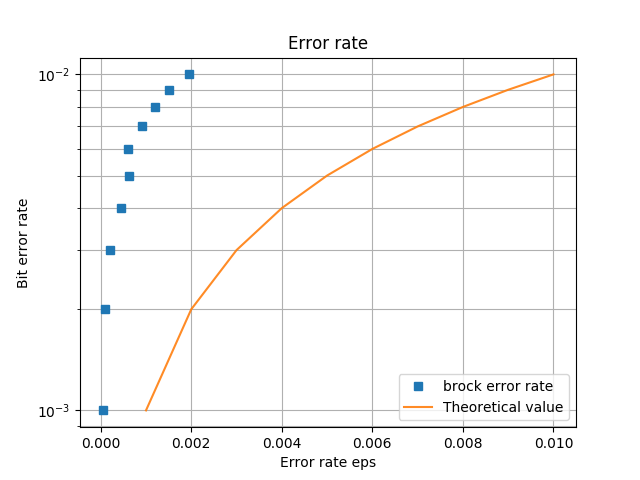
\includegraphics[width=12cm]{./graph2.png}
  \caption{ビット誤り率、ブロック誤り率比較}
\end{figure}



グラフより理論値の乖離度合いはビットを用いたものよりも大きいと
考察されるこれは$k = 4$から$k = 1$になったためと言える。


\section{結論}
通信路モデルにおいてハミング符号を用いた方法を理解できた。

またrandomはそもそもc++のヘッダであり(ヘッダファイルでないことに注意)
c++ であるのになぜ拡張子をc言語にしたかはこれはこの実験の製作者が
c言語、c++に疎いためと推測される。これは来年再来年に学んでいく学生に
有害であるとも推測されるのでここに正しておく。このあたりは評価されたい。


\section{参考文献}
\begin{thebibliography}{9}
  \bibitem{key1} 山本和彦 プログラミングHaskell・オーム社
  \bibitem{key2} 高橋麻奈 やさしいC言語(第5版)・SBクリエイティブ
  \bibitem{key3} 植松友彦 情報理論の考え方 ・講談社
\end{thebibliography}

\section{付録}
実験で使用したプログラムは以下のようになる。
\lstinputlisting[caption = Source.c ,label = program1]{./Source.cpp}

\end{document}
